\chapter{Vergelykings en Ongelykhede}\fancyfoot[LO,RE]{Fokus Area: Wiskunde}
\setcounter{figure}{1}
\setcounter{subfigure}{1}

\section{Oplos van lineêre vergelykings}
\nopagebreak

           
Die eenvoudigste vergelyking om op te los is ’n lineêre vergelyking. ‘n Vergelyking word lineêr genoem indien
die hoogste mag van die veranderlike $1$ is. Die volgende is voorbeelde van lineêre
vergelykings:\par 


\begin{equation*}
\begin{array}{ccl}\hfill 2x+2& =& 1\hfill \vspace{6pt} \\
 \hfill \dfrac{2-x}{3x+1}& =& 2\hfill \vspace{6pt} \\
\hfill 4(2x-9)-4x&=&4-6x \hfill  \vspace{6pt}\\ 
\hfill \dfrac{2a-3}{3}-3a&=&\dfrac{a}{3} \hfill\\
\end{array}
\end{equation*}
% ENGLISH
Solving an equation means finding the value of the variable that makes
the equation true. For example, to solve the simple equation $x+1=1$,
we need to determine the value of $x$ that will make the left hand
side equal to the right hand side. The solution is $x=0$.\par

The solution, also called the root of an equation, is the value of the
variable that satisfies the equation. For linear equations, there is
at most one solution for the equation.\par

To solve equations we use algebraic methods that include expanding
expressions, grouping terms, and factorising. \\
For example,
\begin{equation*}
  \begin{array}{ccll}\hfill 2x+2& =& 1\hfill \\ 
      \hfill 2x& =& 1-2\hfill & \mbox{(groepeer soortgelyke terme saam)}\hfill \\ 
      \hfill 2x& =& -1\hfill & \mbox{(vereenvoudig)}\hfill \\
\hfill x&=& -\frac{1}{2} & \mbox{(deel weerskante met $2$)} \hfill
  \end{array}
\end{equation*}

\begin{equation*}

\end{equation*}
Vervang  $x=-\frac{1}{2}$ in die oorspronklike vergelyking om die antwoord te bevestig:

\begin{equation*}
    \begin{array}{ccl}\hfill \mbox{LK}& =& 2x+2\hfill \\
	  & =& 2(-\frac{1}{2})+2\hfill \\
	  & =& -1+2\hfill \\
	  & =& 1\hfill \\
	  \hfill \mbox{RK}& =& 1\hfill \\
    \end{array}
\end{equation*}
Daarom is $x = -\frac{1}{2}$ 'n geldige oplossing.


\subsection*{Metode: Oplos van lineêre vergelykings}

Die algemene stappe in die oplos van lineêre vergelykings is:
\begin{enumerate}[noitemsep, label=\textbf{\arabic*}. ] 
    \item Verwyder alle hakies in die vergelyking.
    \item Herrangskik die terme van die vergelyking sodat al die terme wat die veranderlike bevat aan een kant van die gelykaanteken is en alle konstantes aan die ander kant.
    \item Groepeer alle soortgelyke terme saam en vereenvoudig so ver as moontlik.
\item Faktoriseer, indien nodig.
    \item Vind die oplossing en skryf die antwoord(e) neer.
    \item Stel die oplossing in die oorspronklike vergelyking in om die antwoord te bevestig.
\end{enumerate}

\textbf{Onthou: } die twee kante van 'n vergelyking moet altyd balanseer; wat jy doen aan die een kant moet jy doen aan die ander kant. 'n moontlike oplossing van NIE de vergelyking bevredig nie, is nie geldig nie.

    
% \begin{wex}{Oplos van lineêre vergelykings}
% {
% Los op vir $x$: $15-2x=3$
% }
% {
% \westep{Herrangskik}
% 
% \begin{equation*}
%     \begin{array}{cclc}\hfill 15-2x& =& 3\hfill & \\
% 	    \hfill -2x& =& 3-15\hfill & \hfill 
% 	    
%     \end{array}
% \end{equation*}
% 
% \westep{Vereenvoudig}
% \begin{equation*}
%     \begin{array}{cccc}\hfill -2x& =&-12\hfill & 
% 	    
%     \end{array}
% \end{equation*}
% 
% \westep{Deel weerskante met $-2$}
% \begin{equation*}
%     \begin{array}{cccc}\hfill x& =&6\hfill & 
% 	    
%     \end{array}
% \end{equation*}
% \westep{Stel die oplossing in die oorspronklike vergelyking in om die antwoord te bevestig.}  
% 
% \begin{equation*}
% \begin{array}{ccc}\hfill 15 - 2(6)& =& 3\hfill \\
%  \hfill 15-12& =& 3\hfill \\
% \hfill 3 &=& 3\hfill
% \end{array}
% \end{equation*}
% Aangesien beide kante gelyk is, is die antwoord korrek
% }
% \end{wex}

\begin{wex}
{Los line\^ere vergelykings op }
{Los op vir $x$: $4(2x-9)-4x=4-6x$}
{
\westep{Brei die hakies uit en vereenvoudig}

\begin{equation*}
    \begin{array}{ccl}\hfill 4(2x-9)-4x& =& 4-6x\hfill  \\ 
	\hfill 8x-36-4x& =& 4-6x\hfill   \\ 
	\hfill 8x-4x+6x& =& 4+36\hfill  \\ 
	\hfill (8x-4x+6x)& =& (4+36)\hfill   \\   
	\hfill 10x& =& 40\hfill  
    \end{array}
\end{equation*}

\westep{Deel weerskante deur $10$}
\begin{equation*}
    \begin{array}{ccl}
	\hfill \dfrac{10}{10}x& =& \dfrac{40}{10}\hfill\\
	\hfill x& =& 4\hfill  
    \end{array}
\end{equation*}

\westep{Stel die oplossing in die oorspronklike vergelyking in}  

\begin{equation*}
    \begin{array}{ccl}\hfill 4[2(4)-9]-4(4)& =& 4-6(4)\hfill \\
	\hfill 4(8-9)-16& =& 4-24\hfill \\
	\hfill 4(-1)-16& =& -20\hfill \\
	\hfill -4-16& =& -20\hfill \\
	\hfill -20& =& -20\hfill 
    \end{array}
\end{equation*}
Aangesien beide kante gelyk is, is die antwoord korrek.
}
\end{wex}

\begin{wex}{Oplos van lineêre vergelykings}
{Los op vir $x$: $\dfrac{2-x}{3x+1}=2$} 
{
\westep{Ons begin deur weerskante van die vergelyking te vermenigvuldig met $(3x+1)$}
Omdat deling met $0$ ontoelaatbaar is, is daar ’n beperking op die waarde van ($x\neq -\frac{1}{3}$).

\begin{equation*}
    \begin{array}{ccll}\hfill \dfrac{2-x}{3x+1}& =& 2\hfill & \\
	\hfill (2-x)& =& 2(3x+1)\hfill & \\ 
    \end{array}
\end{equation*}

\westep{Brei hakies uit en vereenvoudig}
\begin{equation*}
    \begin{array}{ccll}
	\hfill 2-x& =& 6x+2\hfill & \hfill \\ 
	\hfill -x-6x& =& 2-2\hfill & \hfill \\ 
	\hfill -7x& =& 0\hfill & \hfill
    \end{array}
\end{equation*}

\westep{Deel weerskante deur $-7$}
\begin{equation*}
    \begin{array}{ccll}

	\hfill x& =& \dfrac{0}{-7}\hfill & \\
	\hfill x& =& 0\hfill & \hfill 
    \end{array}
\end{equation*}
Let op dat $0$ gedeel deur enige ander getal is $0$.

\westep{Stel die oplossing in die oorspronklike vergelyking in:}

\begin{equation*}
    \begin{array}{ccc}\hfill \dfrac{2-(0)}{3(0)+1}& =& 2\hfill \vspace{6pt}\\
	\hfill 2& =& 2\hfill 
\end{array}
\end{equation*}
Aangesien weerskante gelyk is, is die antwoord korrek.
}
\end{wex}


\begin{wex}
{Oplos van lineêre vergelykings}
{Los op vir $a$: $\dfrac{2a-3}{3}-3a=\dfrac{a}{3}$}
{
\westep{Begin deur elk van die terme in die vergelyking te vermenigvuldig met  $3$ en vervolgens te vereenvoudig}  

\begin{equation*}
    \begin{array}{cccc}\hfill 2a-3 - 9a &= &a\hfill & \\ 
\hfill -7a - 3 &= &a\hfill & 
    \end{array}
\end{equation*}

\westep{Herrangskik en vereenvoudig}
\begin{equation*}
    \begin{array}{cccc}\hfill -7a -a &= &3\hfill & \\ 
\hfill -8a &= &3\hfill & \\
    \end{array}
\end{equation*}

\westep{Deel weerskante deur $-8$} 
\begin{equation*}
    \begin{array}{cccc}\hfill a &= & -\dfrac{3}{8}\hfill & \\ 

    \end{array}
\end{equation*}

\westep{Stel die oplossing in die oorspronklike vergelyking in}
\begin{equation*}
    \begin{array}{ccll}\hfill \dfrac{2(-\frac{3}{8}) - 3}{3} - 3(-\frac{3}{8}) &= & \dfrac{-\frac{3}{8}}{3}\hfill & \\ 
\\
      \hfill \dfrac{(-\frac{3}{4}) - \frac{12}{4}}{3} + \frac{9}{8} &= & \dfrac{-\frac{3}{8}}{3}\hfill & \\ 
\\
 \hfill \Bigg[-\frac{15}{4} \times \frac{1}{3}\Bigg] + \frac{9}{8} &= & -\frac{3}{8} \times \frac{1}{3}\hfill & \\ 
\\
 \hfill -\frac{5}{4} + \frac{9}{8} &= & -\frac{1}{8}\hfill & \\ 
 \hfill -\frac{10}{8} + \frac{9}{8} &= & -\frac{1}{8}\hfill & \\ 
 \hfill -\frac{1}{8} &= & -\frac{1}{8}\hfill & 
    \end{array}
\end{equation*}
Beide kante is gelyk, dus die oplossing is reg.
}
\end{wex}


\begin{exercises}{}
% ENGLISH in sentence below
{Oplos van lineêre vergelykings (Aanvaar alle noemers is non-zero):

\begin{multicols}{2}
\begin{enumerate}[itemsep=6pt, label=\textbf{\arabic*}. ] 
\item   $2y-3=7$
\item   $-3y=0$        
\item   $16y+4=-10$        
\item   $12y+0=144$
\item   $7+5y=62$       
\item  $55=5x+\dfrac{3}{4}$ 
\item   $5x=2x+45$        
\item  $23x-12=6+3x$
\item   $12-6x+34x=2x-24-64$
\item   $6x+3x=4-5(2x-3)$
\item   $18-2p=p+9$   
\item   $\dfrac{4}{p}=\dfrac{16}{24}$
\item   $-(-16-p)=13p-1$
\item   $3f-10=10$
\item   $3f+16=4f-10$
\item   $10f+5=-2f-3f+80$
\item   $8(f-4)=5(f-4)$
\item  $6=6(f+7)+5f$      
\item $(a-1)^{2} - 2a = (a+3)(a-2) - 3$
\item $-7x = x+8(1-x)$ 
\item $5-\dfrac{7}{b} = \dfrac{2(b+4)}{b}$
\item $\dfrac{x+2}{4} - \dfrac{x-6}{3} = \dfrac{1}{2}$
\item $ 3 - \dfrac{y-2}{4} = 4$
\item $ \dfrac{a+1}{a+2} = \dfrac{a-3}{a+1}$
\item $(x-3)(x+2)=x(x-4)$
\item $1,5x+3,125=1,25x$
\item $\frac{1}{3}P + \frac{1}{2}P - 10 = 0$
\item $1 \frac{1}{4} (x-1)-1\frac{1}{2}(3x+2)=0$
\item $\frac{5}{2a}+\frac{1}{6a}-\frac{3}{a}=2$
\item $\frac{3}{2x^2}+\frac{4}{3x}-\frac{5}{6x}=0$  
\end{enumerate}
\end{multicols}
\practiceinfo
\par 
\par \begin{tabular}[h]{cccccc}
(1.-5.) 00dn&  (6.-10.) 00dp&  (11.-15.) 00dq&  (16.-20.) 00dr& (21.-24) 00md & (25.-30.) 022t & \end{tabular}
}
\end{exercises}


% \begin{exercises}{}
% {
% Oplos van lineêre vergelykings (Aanvaar alle noemers is non-zero):
% \begin{multicols}{2}
% \begin{enumerate}[noitemsep, label=\textbf{\arabic*}. ] 
% \item   $2y-3=7$
% \item   $-3y=0$        
% \item   $16y+4=-10$        
% \item   $12y+0=144$
% \item   $7+5y=62$   \vspace{6pt}     
% \item  $55=5x+\dfrac{3}{4}$ \vspace{6pt}
% \item   $5x=2x+45$        
% \item  $23x-12=6+3x$
% \item   $12-6x+34x=2x-24-64$
% \item   $6x+3x=4-5(2x-3)$
% \item   $18-2p=p+9$   \vspace{6pt}
% \item   $\dfrac{4}{p}=\dfrac{16}{24}$
% \item   $-(-16-p)=13p-1$
% \item   $3f-10=10$
% \item   $3f+16=4f-10$
% \item   $10f+5=-2f-3f+80$
% \item   $8(f-4)=5(f-4)$
% \item  $6=6(f+7)+5f$      
% \item $(a-1)^{2} - 2a = (a+3)(a-2) - 3$
% \item $-7x = x+8(1-x)$ \vspace{6pt}
% \item $5-\dfrac{7}{b} = \dfrac{2(b+4)}{b}$\vspace{6pt}
% \item $\dfrac{x+2}{4} - \dfrac{x-6}{3} = \dfrac{1}{2}$\vspace{6pt}
% \item $ 3 - \dfrac{y-2}{4} = 4$\vspace{6pt}
% \item $ \dfrac{a+1}{a+2} = \dfrac{a-3}{a+1}$
%   
% \end{enumerate}
% \end{multicols}
% 
% \insertpracticeinfo{24}
% }
% \end{exercises}

\section{Oplos van kwadratiese vergelykings}

’n Kwadratiese vergelyking, is ’n vergelyking waar die mag van die veranderlike hoogstens
$2$ is. \\Die volgende is voorbeelde van kwadratiese vergelykings:\par 


\begin{equation*}
    \begin{array}{ccl}\hfill 2{x}^{2}+2x& =& 1\hfill \\
	\hfill 3{x}^{2}+2x-1&=&0 \\ 
	\hfill 0&=&-2{x}^{2}+4x-2\hfill 
    \end{array}
\end{equation*}

Kwadratiese vergelykings verskil van lineêre vergelykings daarin dat ’n lineêre vergelyking slegs een oplossing
het, terwyl ‘n kwadratiese vergelyking hoogstens 2 oplossings het. Daar is spesiale gevalle waar ’n kwadratiese
vergelyking slegs een oplossing het.\par


Ons kan 'n kwadratiese vergelyking oplos deur faktorisering te gebruik. Byvoorbeeld, om $2{x}^{2}-x-3 = 0$ op te los, moet ons die uitdrukking in sy ekwivalente gefaktoriseerde vorm skryf as $(x+1)(2x-3)=0$.\par

\mindsetvid{Graphs and quadratic equations}{VMaec}
% \begin{activity}{}
% Los die Kwadratiese Vergelykings $x^{2}=16$ op deur drie verskillende metodes te gebruik:
% \begin{enumerate}[noitemsep, label=\textbf{\arabic*}. ] 
% \item Inspeksie (probeer en toets)
% \item Trek die vierkantswortels
% \item Faktorisering
% \end{enumerate}
% (Let op, indien $a \times b = 0$ dan $a = 0$ of $b=0$)
% \end{activity}



\subsection*{Metode: Oplos van kwadratiese vergelykings}
\begin{enumerate}[noitemsep, label=\textbf{\arabic*}. ] 
\item Skryf die vergelyking die vorm $ax^{2} +bx +c =0$.
\item Deel heel eerste die hele vergelyking deur enige gemene faktore van die koëffisiënte, ten einde ’n vergelyking te kry van die vorm $a{x}^{2}+bx+c=0$ waar $a$, $b$ en
$c$ geen gemeenskaplike faktore het nie. Byvoorbeeld $2{x}^{2}+4x+2=0$ kan geskryf word as
${x}^{2}+2x+1=0$, deur te deel met $2$.
\item Skryf $a{x}^{2}+bx+c=0$ in terme van sy faktore  $(rx+s)(ux+v)=0$.

\item Die twee oplossings is $(rx+s)=0$ of $(ux+v)=0$, dus $x = -\dfrac{s}{r}$ of $x=-\dfrac{v}{u}$.
\item Vervang elke moontlike waarde van die oplossing in die oorspronklike vergelyking in om te toets of dit ’n
geldige oplossing is.

\end{enumerate}

        
\begin{wex}
{Oplos van kwadratiese vergelykings }
{Los op vir $x$: $3{x}^{2}+2x-1=0$}
{
\westep{Die vergelyking is alreeds n die regte vorm ${ax}^{2} + bx + c = 0$}

\westep{Faktoriseer}
\begin{equation*}
(x+1)(3x-1)=0
\end{equation*}

\westep{Los op vir beide wortels}
Ons het
\begin{equation*}
     \begin{array}{ccc}\hfill x+1&=&0\hfill \\
	\hfill \therefore x&=&-1
    \end{array}
\end{equation*}

OF
\begin{equation*}
     \begin{array}{ccc}\hfill 3x-1&=&0\hfill \\
	\hfill \therefore x&=&\frac{1}{3}
    \end{array}
\end{equation*}
\westep{Kontroleer beide antwoorde deur instelling in die oorspronklike vergelyking}
\westep{Skryf die finale antwoord}
Die oplossing van $3{x}^{2}+2x-1=0$ is dus $x=-1$ of $x=\frac{1}{3}$.
}
\end{wex}


\begin{wex}{ Oplos van kwadratiese vergelykings }
{ Vind die wortels van: $0=-2{x}^{2}+4x-2$}
{
%ENGLISH in westep below
\westep{Deel weerskante van die vergelyking deur common factor $-2$}

\begin{equation*}
\begin{array}{ccc}\hfill -2{x}^{2}+4x-2& =& 0\hfill \\ \hfill {x}^{2}-2x+1& =& 0\hfill \end{array}
\end{equation*}

\westep{Die vergelyking is in die regte vorm ${ax}^{2} + bx + c = 0$}

\westep{Faktoriseer}
\begin{equation*}
\begin{array}{ccc} \hfill (x-1)(x-1) &=& 0 \hfill \\
\hfill (x-1)^{2} &=&0 \hfill 
\end{array}
\end{equation*}

\westep{Die kwadratiese uitdrukking is ’n volkome vierkant}
Hierdie is a voorbeeld van 'n spesiale situasie waar daar net een oplossing vir die kwadratiese vergelykings is
\begin{equation*}
\begin{array}{ccc} \hfill x -1 &=& 0 \hfill \\
\hfill \therefore x &=&1 \hfill 
\end{array}
\end{equation*}

\westep{Stel die oplossing in die oorspronklike vergelyking in om dit te toets}

 
\westep{Skryf die finale antwoord}
Die oplossing van $0=-2{x}^{2}+4x-2$ is $x=1$.
}
\end{wex}


\begin{exercises}{}
%ENGLISH below
{Solve the following equations:
\begin{multicols}{2}
\begin{enumerate}[itemsep=5pt, label=\textbf{\arabic*}. ] 
\item  $9x^{2}-6x-8=0$%$(3x+2)(3x-4)=0$
\item  $5x^{2}-21x-54=0$%$(5x-9)(x+6)=0$
\item  $4y^{2}-9=0$%$(2y+3)(2y-3)=0$ 
\item  $4x^{2}-16x-9=0$%$(2x+1)(2x-9)=0$    
\item  $4x^{2}-12x=-9$%$(4x)(x-3)=-9$       
\item  $20m+25{m}^{2}=0$
\item  $2{x}^{2}-5x-12=0$  
\item  $-75{x}^{2}+290x=240$
\item  $2x=\frac{1}{3}{x}^{2}-3x+14\frac{2}{3}$
\item  ${x}^{2}-4x=-4$      
\item  $-{x}^{2}+4x-6=4{x}^{2}-14x+3$       
\item  ${t}^{2}=3t$  
\item  ${x}^{2}-10x=-25$      
\item  ${x}^{2}=18$
\item  ${p}^{2}-6p=7$
\item  $4{x}^{2}-17x-77=0$
\item  $14{x}^{2}+5x=6$
\item  $2{x}^{2}-2x=12$  
\item  $\frac{a+1}{3a-4}+\frac{9}{2a+5}+\frac{2a+3}{2a+5}=0$
\item  $\frac{3}{9a^2-3a+1}-\frac{3a+4}{27a^3+1}=\frac{1}{9a^2-1}$          
\end{enumerate}
\end{multicols}
\practiceinfo
\par 
\par\begin{tabular}[h]{cccccc}
(1.-5.) 00ds&  (6.-11.) 00dt&  (12.-18.) 00du & (19.-20.) 022u &\end{tabular}
}
\end{exercises}


\section{Oplos van gelyktydige vergelykings}


Tot dusver het alle vergelykings slegs een onbekende veranderlike gehad wat ons moes vind.
Wanneer twee onbekendes bepaal moet word, het ons twee vergelykings nodig. Hierdie vergelykings word gelyktydige vergelykings
genoem. Die oplossing vir die stelsel van gelyktydige vergelykings is die waardes van die veranderlikes wat die stelsel van vergelykings gelyktydig sal bevredig. In die algemeen beteken dit indien daar $n$ onbekende veranderlikes is, benodig ons $n$ vergelykings om ’n oplossing vir elk van die $n$ veranderlikes te vind.\par 
’n Voorbeeld van stel gelyktydige vergelykings is:

\begin{equation*}
\begin{array}{rcl} x+y&=&-1 \\ 
 3&=&y-2x 
\end{array}
\end{equation*}

%ENGLISH
We have two independent equations to solve for two unknown variables. We can solve simultaneous equations algebraically using substitution and elimination methods. We will also show that a system of simultaneous equations can be solved graphically.\par 
\par 
      

\mindsetvid{What are simultaneous equations}{VMaex}

\subsection*{Oplossing deur vervanging}
\begin{itemize}
 \item Probeer om een van die vergelykings op te los vir een van die veranderlikes.
\item Vervang die resultaat in die ander vergelykings. Deur dit te doen verminder die hoeveelheid
vergelykings en ook die hoeveelheid onbekende veranderlikes met 1.
\item Hierdie proses word herhaal tot ‘n enkele vergelyking met 1 veranderlike oorbly, wat (hopelik) opgelos kan word.
\item Vervang heirdie oplossing terug in die oorspronklike vergelyking om die waarde te vind van die ander onbekende veranderlike.
\end{itemize}

% \Note{As die vraag nie spesifiek vra vir 'n grafiese oplossing nie, behoort die stelsel van gelyktydige vergelykings algebra\"ies opgelos te word.}
\begin{wex}
{Gelyktydige vergelykings}
%ENGLISH below
{Solve for $x$ and $y$:
\begin{align*}
  x-y &= 1 ~~~\ldots \ldots \ldots \ldots (1)\\
  3 &= y-2x \ldots \ldots \ldots (2)
\end{align*}
}
{
\westep{Use equation $(1)$ to express $x$ in terms of $y$}
\begin{equation*}
  x = y+1
\end{equation*}

\westep{Substitute $x$ into equation $(2)$ and solve for $y$}
\begin{align*}
  3 &= y-2(y+1) \\
  3 &= y - 2y - 2 \\
  5 &= -y \\
  \therefore y &= -5
\end{align*}

\westep{Substitute $y$ back into equation $(1)$ and solve for $x$}
\begin{align*}
  x &= (-5) + 1 \\
  \therefore x &= -4
\end{align*}

\westep{Toets oplossing deur instelling in beide oorspronklike vergelykings}  

\westep{Skryf die finale antwoord}
\begin{align*}
x &= -4\\  
y &= -5 
  
\end{align*}
}
\end{wex}

%ENGLISH in wex below
\begin{wex}
{Gelyktydige vergelykings}
{
Los die volgende stelsel gelyktydige vergelykings op:
\begin{equation*}
\begin{array}{ccc}
  4y+3x &= 100  ~~\ldots \ldots \ldots \ldots (1) \\
  4y - 19x &= 12 ~~~~\ldots \ldots \ldots \ldots (2)
\end{array}
\end{equation*}
}
{
\westep{Gebruik een van die vergelukings om $x$ uit te druk in terme van $y$}
\begin{equation*}
    \begin{array}{ccl}\hfill 4y+3x & =& 100\hfill \\
\hfill 3x &=& 100 - 4y \hfill \\
\hfill x& =& \dfrac{100 - 4y}{3} \hfill
    \end{array}
\end{equation*}


\westep{Substitute $x$ into equation $(2)$ and solve for $y$}
\begin{equation*}
    \begin{array}{ccl}\hfill 4y - 19(\dfrac{100 - 4y}{3})& =& 12\hfill \\
	\hfill 12y - 19(100 - 4y)  & =& 36\hfill \\
	\hfill 12y - 1900 + 76y & =& 36 \hfill \\
\hfill  88y& =& 1936 \hfill \\
\hfill \therefore y& =& 22 \hfill
    \end{array}
\end{equation*}

\westep{Substitute $y$ back into equation $(1)$ and solve for $x$}
\begin{equation*}
    \begin{array}{ccl}\hfill x &=& \dfrac{100 - 4(22)}{3}\hfill \vspace{6pt}\\
	\hfill & =& \dfrac{100-88}{3}\hfill \vspace{6pt}\\
	\hfill & =& \dfrac{12}{3}\hfill\vspace{6pt} \\
	\hfill \therefore x&=& 4 \hfill 
    \end{array}
\end{equation*}

\westep{Toets die oplossing deur instelling in beide oorspronklike vergelykings}  

\westep{Skryf die finale antwoord}
\begin{equation*}
\begin{array}{ccc}
 \hfill x& =& 4\hfill \\
\hfill y& =& 22\hfill 
\end{array}
\end{equation*}
}
\end{wex}

\subsection*{Los op deur eliminasie}

\begin{wex}
{Gelyktydige vergelukings}
{
Los die volgende stelsel van vergelykings op:
\begin{align*}
  3x+y &= 2  ~~~\ldots \ldots \ldots \ldots (1)\\
  6x-y &= 25 ~~\ldots \ldots \ldots \ldots (2)
\end{align*}
}
{
\westep{Maak die ko\"effisi\"ente van een van die veranderlikes dieselfde in beide vergelykings}
Die ko\"effisie\"ente van $y$ is $1$ en $-1$. Elimineer die veranderlike $y$ deur die twee vergelykings bymekaar te tel:
\begin{equation*}
\begin{array}{ccll}\hfill & 3x+y& =& 2\hfill \\ 
\hfill+ & 6x-y& =& 25\hfill \\ \hline
 \hfill & 9x + 0 &=& 27
\end{array}
\end{equation*}


\westep{Vereenvoudig en los op vir $x$}
\begin{equation*}
    \begin{array}{ccl}\hfill 9x& =& 27\hfill \\
	\hfill \therefore x  & =& 3\hfill 
    \end{array}
\end{equation*}

\westep{Vervang die waarde van $x$ terug in enige van die oorspronklike vergelykings en los op vir $y$}
\begin{equation*}
    \begin{array}{ccl}\hfill 3(3) + y &=& 2\\
	\hfill y & =& 2-9\\
	\hfill \therefore y & =& -7 
   \end{array}
\end{equation*}

\westep{Kontroleer dat die oplossing $x=3$ en $y=-7$ albei die oorspronklike vergelykings bevredig}  

\westep{Skryf die finale antwoord}
\begin{equation*}
\begin{array}{ccc}
 \hfill x& =& 3\hfill \\
\hfill y& =& -7\hfill 
\end{array}
\end{equation*}
}
\end{wex}

%English below
\begin{wex}
{Gelyktydige vergelykings}
{
Los die volgende stel gelyktydige vergelykings op:
\begin{align*}
  2a - 3b &= 5 ~~~~\ldots \ldots \ldots \ldots (1) \\
  3a-2b &= 20 ~~~\ldots \ldots \ldots \ldots (2)
\end{align*}
}
{
\westep{Maak die ko\"effisi\"ente van enige van die veranderlikes dieselfde in beide vergelykings}
By multiplying equation $(1)$ by $3$ and equation $(2)$ by $2$, both coefficients of $a$ will be $6$.
\begin{equation*}
\begin{array}{cccc}\hfill & 6a-9b& =& 15\hfill \\ 
\hfill- & (6a-4b& =& 40)\hfill \\ \hline
 \hfill & 0 - 5b &=& -25 

\end{array}
\end{equation*}
(Wees versigtig met die teken as die een vergelyking van die ander afgetrek word.)

\westep{Vereenvoudig en los op vir $b$}
\begin{equation*}
    \begin{array}{ccl}
 \hfill b &=& \dfrac{-25}{-5} \\
 \hfill \therefore b &=& 5
    \end{array}
\end{equation*}

\westep{Vervang die waarde van $b$ terug in enige van die oorspronklike vergelykings in en los op vir  $a$}
\begin{equation*}
    \begin{array}{ccl}\hfill 2a - 3(5)&=& 5\\
	\hfill 2a-15 & =& 5\\
	\hfill 2a & =& 20\\
	\hfill \therefore a & =& 10 
   \end{array}
\end{equation*}

\westep{Toets dat die oplossing $a=10$ en $b=5$ beide oorspronklike vergelykings bevredig}  

\westep{Skryf die finale antwoord}
\begin{equation*}
\begin{array}{ccc}
 \hfill a& =& 10\hfill \\
\hfill b& =& 5\hfill 
\end{array}
\end{equation*}
}
\end{wex}


\subsection*{Grafiese oplossing}

Gelyktydige vergelykings kan ook grafies opgelos word. Die oplossing van die gelyktydige vergelykings word gegee
deur die koördinate van die punt waar die twee grafieke mekaar sny.\par 
Byvoorbeeld:
\begin{align*}
  x &= 2y  ~\ldots \ldots \ldots \ldots \ldots (1)\\  
  y &= 2x-3  \ldots \ldots \ldots \ldots (2)
\end{align*}

%english
The graphs of the two equations are shown below.\\\par 

\setcounter{subfigure}{0}
\begin{figure}[H] % horizontal\label{m39257*uid96}
\begin{center}
% \rule[.1in]{\figurerulewidth}{.005in} \\

\begin{pspicture}(-3,-2)(4,2)
% \psgrid[gridcolor=lightgray,gridlabels=0,gridwidth=0.5pt]
\psaxes[dx=1,Dx=1,arrows=<->](0,0)(-3,-2)(4,2)
\pstextpath[c](-1.1,-0.3){\psplot[xunit=1,plotstyle=curve,arrows=<->]{0.5}{2.5}{x 2 mul 3 sub}}{\small{$y=2x-3$}}
\pstextpath[c](1.5,-0.3){\psplot[xunit=1,plotstyle=curve,arrows=<->]{-1}{3.5}{0.5 x mul}}{\small{$y=\frac{1}{2}x$}}
\uput[l](2,1.1){$(2,1)$}
\psdot(2,1)
\end{pspicture}

% \vspace{2pt}
% \vspace{.1in}
% \rule[.1in]{\figurerulewidth}{.005in} \\
\end{center}
\end{figure}       
Die snypunt van die 2 grafieke is $(2;1)$. Dus, die oplossing van die stel gelyktydige vergelykings in $x=2$ en $y=1$.
Dit kan ook algebraïes gevind word. 
Stel vegelyking $(1)$ in vergelyking $(2)$ in:

\begin{equation*}
\begin{array}{ccl}\hfill x& =& 2y\hfill \\
 \hfill y& =& 2(2y)-3\hfill 
\end{array}
\end{equation*}
Los op vir $y$:
\begin{equation*}
\begin{array}{ccl}
 \hfill y-4y& =& -3\hfill \\
 \hfill -3y& =& -3\hfill \\ 
\hfill \therefore y& =& 1\hfill 
\end{array}
\end{equation*}
Stel die antwoord vir $y$ terug in vergelyking $(1)$ in:
\begin{equation*}
\begin{array}{ccl}
 \hfill x& =& 2(1)\hfill \\
 \therefore x&=& 2\hfill \end{array}
\end{equation*}

Let daarop dat beide metodes dieselfde oplossing gee.

\begin{wex}
{Gelyktydige vergelykings }
{Los die volgende stel gelyktydige vergelykings grafies op:
\begin{align*}
  4y+3x &= 100 \ldots \ldots \ldots \ldots (1)\\
  4y-19x &= 12 ~~\ldots \ldots \ldots \ldots (2)
\end{align*}
}
{
\westep{Skryf albei vergelykings in die vorm $y=mx+c$}  

\begin{equation*}
\begin{array}{ccl}\hfill 4y+3x& =& 100\hfill \\
 \hfill 4y& =& 100-3x\hfill \\
 \hfill y& =& -\dfrac{3}{4}x + 25\hfill \end{array}
\end{equation*}
\\
\begin{equation*}
\begin{array}{ccl}\hfill 4y-19x& =& 12\hfill \\ \hfill 4y& =& 19x+12\hfill \\ \hfill y& =& \dfrac{19}{4}x+3\hfill \end{array}
\end{equation*}



\westep{Skets die grafieke van die 2 vergelykings op dieselfde assestelsel}
\setcounter{subfigure}{0}
\begin{figure}[H] % horizontal\label{m39257*id159679}
\begin{center}
% \label{m39257*id159679!!!underscore!!!media}\label{m39257*id159679!!!underscore!!!printimage}
%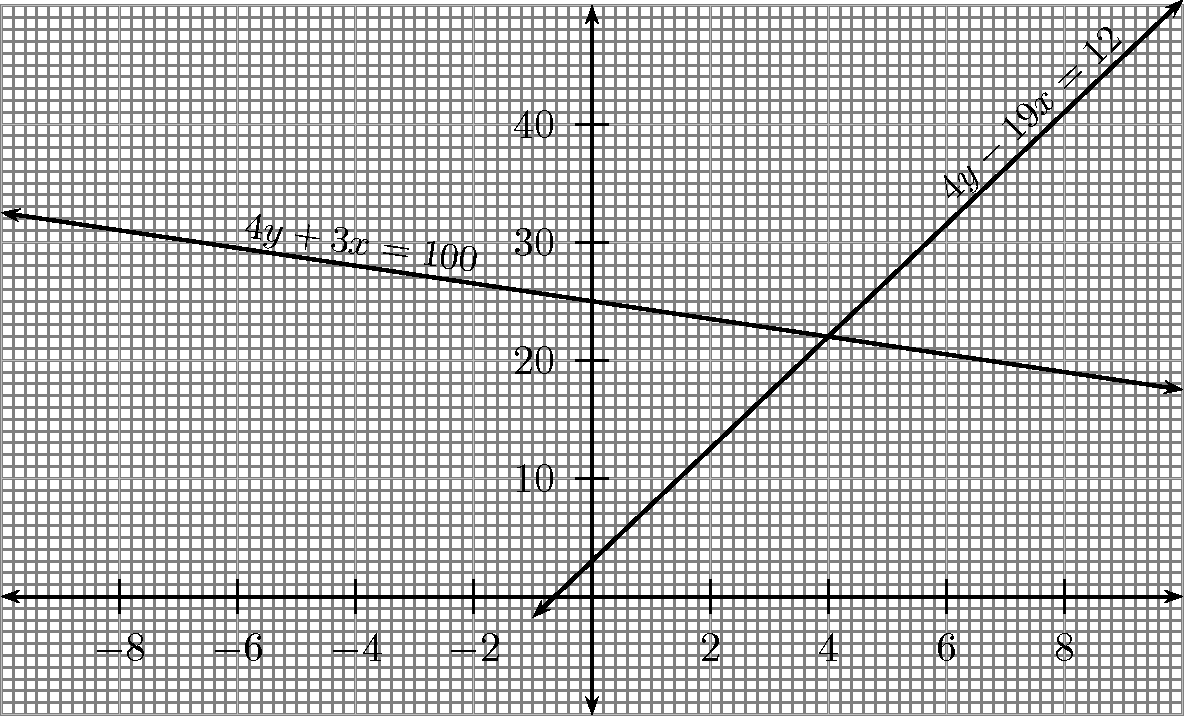
\includegraphics{col11306.imgs/m39257_MG10C10_007.png} % ;MG10C10\_007.png;;;6.0;8.5;
\begin{center}
\begin{pspicture}(-5,-1)(5,5)
%  \psgrid[subgriddiv=10,gridcolor=lightgray,gridlabels=0,gridwidth=0.1pt]
\psaxes[dx=1,dy=1,Dy=10,Dx=2,arrows=<->](0,0)(-5,-1)(5,5)
\pstextpath[c](-2,0.1){\psplot[xunit=0.5,yunit=0.1,plotstyle=curve,arrows=<->]{-10}{10}{0.75 x mul neg 25 add}}{\small{$4y+3x=100$}}
\pstextpath[c](2.2,0.1){\psplot[xunit=0.5,yunit=0.1,plotstyle=curve,arrows=<->]{-1}{10}{4.75 x mul 3 add}}{\small{$4y-19x=12$}}
\end{pspicture}
\end{center}

% \vspace{2pt}
% \vspace{.1in}
\end{center}
\end{figure}         

\westep{Vind die snypunt van die twee grafieke}
Die twee grafieke sny by $(4;22)$ 

\westep{Skryf die finale antwoord}
\begin{equation*}
\begin{array}{ccl}\hfill x& =& 4\hfill \\ \hfill y& =& 22\hfill \end{array}
\end{equation*}

}
\end{wex}

%English below
\begin{exercises}{}
{
% \Note{Solving a system of simultaneous equations graphically is sometimes not very accurate but provides a valuable method of solution.}
\begin{enumerate}[noitemsep, label=\textbf{\arabic*}. ] 
\item Solve for $x$ and $y$: 
\begin{enumerate}[noitemsep, label=\textbf{(\alph*)} ] 
\item $3x-14y=0$ and $x-4y+1=0$
\item $x+y=8$ and $3x + 2y = 21$
\item $y=2x+1$ and $x + 2y + 3 = 0$
\item $\frac{a}{2}+b=4$ and $\frac{a}{4} -\frac{b}{4}=1$
\item $\frac{1}{x}+\frac{1}{y}=3$ and $\frac{1}{x}-\frac{1}{y}=11$
\end{enumerate}

\item Solve graphically and check your answer algebraically:

\begin{enumerate}[noitemsep, label=\textbf{(\alph*)} ] 

\item  $x+2y=1$ and $\frac{x}{3} + \frac{y}{2} = 1$
\item $5= x+y$ and $x = y-2$
\item $3x - 2y = 0$ and $x - 4y + 1 = 0$
\item $\frac{x}{4}=\frac{y}{2}-1$  and $\frac{y}{4}+\frac{x}{2}=1$
\item $2x+y=5$ and $3x-2y=4$
\end{enumerate}
\end{enumerate}
\practiceinfo
\par 
\par \begin{tabular}[h]{cccccc}
(1.a-e) 00dv&  (2a-e.) 00dw & \end{tabular}
}
\end{exercises}

\section{Woordprobleme}

%english
To solve word problems we need to write a set of equations that represent the problem mathematically. 
The solution of the equations is then the solution to the problem.


\subsection*{Strategie vir die oplos van probleme}

\begin{enumerate}[noitemsep, label=\textbf{\arabic*}. ] 
\item Lees die hele vraag.
\item Bepaal wat gevra word.
\item Gebruik ’n veranderlike om die onbekende getalle/hoeveelhede word voor te stel, $x$.
\item  Herskryf die inligting wat gegee is in terme van die veranderlike. Dus, vertaal die woorde in algebraïese
taal.
\item Stel ’n vergelyking of ’n stel gelyktydige vergelykings op om die onbekende te kry.
\item Los die vergelyking algebraïes op om die oplossing te vind.
\item Toets die oplossing.
\end{enumerate}

\mindsetvid{Balancing equations}{VMafb}

\begin{wex}
{Oplos van woordprobleme}
{
%english below
 ’n Winkel verkoop tweewielfietse en driewiele. In totaal is daar $7$ fietse (fietse sluit tweewielfietse en driewiele in) en $19$ wiele. Bepaal hoeveel van elke soort fiets daar is, if a bicycle has two wheels and a tricycle has three wheels.
}
{
\westep{Ken veranderlike toe aan die onbekende}
Laat $b$ die aantal tweewielfietse wees  \\
en laat $t$  die aantal driewiele wees. 

\westep{Set up the equations}
\begin{align*}
  b + t &= 7 ~~\ldots \ldots \ldots \ldots (1)\\
  2b + 3t &= 19 \ldots \ldots \ldots \ldots (2)
\end{align*}

\westep{Rearrange equation $(1)$ and substitute into equation $(2)$ }
\begin{align*}
  t &= 7-b \\
  \therefore 2b + 21 - 3b &= 19 \\
  -b &= -2 \\
  \therefore b &= 2
\end{align*}

\westep{Calculate the number of tricycles $t$}
\begin{align*}
  t &= 7-b \\
    &= 7-2 \\
    &= 5
\end{align*}

\westep{Skryf die finale antwoord}
Daar is $5$ driewiele en $2$ fietse.
}       
\end{wex}

\begin{wex}{Oplos van woordprobleme}{
Bongani en Jane is vriende. Bongani vat Jane se fisika toets en wil nie vir haar s\^e wat haar punt is nie. Hy weet Jane hou nie baie van wiskunde nie en besluit om haar te terg. Bongani s\"e 
'ek het $2$ punte meer as jy en ons twee saam het $14$, wat is ons punte?'}
{
\westep{Ken veranderlikes toe aan die onbekendes}
Ons het twee onbekendes. Bongani se punt en Jane se punt 
\\Gestel Bongani het $b$ en Jane het $j$ punte. 

\westep{Stel 'n sisteem van vergelykings op}
\\Bongani het $2$ meer as Jane.
\begin{equation*}
  b=j+2 ~~\ldots \ldots \ldots \ldots (1)
\end{equation*}

Saam her hulle $14$ punte.

\begin{equation*}
  b+j=14 ~~\ldots \ldots \ldots \ldots (2)
\end{equation*}

\westep{Gebruik vergelyking $(1)$ om $b$ uit te druk in terme van $j$}
\begin{equation*}
t=j+2
\end{equation*}

\westep{Vervang in vergelyking $(2)$ in}
\begin{equation*}
    \begin{array}{ccc}\hfill t+j& =& 14\hfill \\
	\hfill (j+2)+j& =& 14\hfill \\

    \end{array}
\end{equation*}

\westep{Herrangskik en los op vir $j$}
\begin{equation*}
    \begin{array}{ccl}\hfill 2j& =& 14 - 2\hfill \\
	\hfill \therefore 2j& =& 12\hfill \\
\hfill \therefore j &=& 6 \hfill

    \end{array}
\end{equation*}

 \westep{Vervang die waarde van $j$ terug in vergelyking $(1)$ en los op vir $b$}
\begin{equation*}
\begin{array}{ccl}\hfill t& =& j+2\hfill \\ & =& 6+2\hfill \\ & =& 8\hfill \end{array}
\end{equation*}
\\
\westep{Kontroleer dat die oplossng beide oorspronklike vergelykings bevredig}
\westep{Skryf die finale antwoord}
Bongani het $8$ punte en Jane het  $6$ punte vir die toets gekry.\\
}
\end{wex}

\begin{wex}
{Oplos van woordprobleme}
{
’n
Vrugteskommel kos R$~2,00$ meer as ’n sjokolade melkskommel. As $3$ vrugteskommels en $5$ sjokolade melkskommels saam,  R$~78,00$ kos,
bepaal die afsonderlike pryse.}

{
\westep{Ken veranderlikes toe aan die onbekendes}  
Gestel die prys van ’n sjokelade melkskommel is $x$ 
\\ rand en die prys van ’n vrugteskommel is  $y$ rand.


\westep{Stel 'n sisteem van vergelykings op}
\begin{align*}
  y &= x+2  \ldots \ldots \ldots (1)\\
  3y+5x &= 78 \ldots \ldots \ldots \ldots (2)
\end{align*}

\westep{Vervang vergelyking $(1)$ in die vergelyking $(2)$ in}
\begin{equation*}
\begin{array}{ccl}\hfill 3(x+2)+5x& =& 78\hfill \\
\end{array}
\end{equation*}

\westep{Herrangskik en los op vir $x$}
\begin{equation*}
\begin{array}{ccl}
 \hfill 3x+6+5x& =& 78\hfill \\ 
\hfill 8x& =& 72\hfill \\ 
\hfill \therefore x& =& 9\hfill \\  \end{array}
\end{equation*}

\westep{Vervang die waarde van $x$ terug in vergelyking $(1)$ in en los op vir $y$}
\begin{equation*}
\begin{array}{ccl}
\hfill y& =& x+2\hfill \\
 \hfill & =& 9+2\hfill \\ 
\hfill & \therefore =& 11\hfill  \end{array}
\end{equation*}
\westep{Kontroleer dat die oplossing beide oorspronklike vergelykings bevredig}
\westep{Skryf die finale antwoord}
Een sjokelade melkskommel kos R$~9,00$ en een vrugteskommel
kos R$~ 11,00$.
}
\end{wex}

\begin{wex}
{Oplos van woordprobleme}
{
Die produk van twee opeen volgende negatiewe heelgetalle is $1~122$. Vind die twee heelgetalle.
} 
{
\westep{Ken veranderlikes toe aan die onbekendes}
Gestel die eerste heelgetal is $n$ 
\\Dan is die tweede heelgetal $n+1$.\par 

\westep{Stel 'n vergelyking op}  
\begin{equation*}
\begin{array}{cll}\hfill n(n+1)& =& ~1122\hfill \end{array}
\end{equation*}

\westep{Brei uit en los op vir $n$}
\begin{equation*}
    \begin{array}{cll}
	\hfill n^{2} + n =& 1~122\hfill \\
\hfill n^{2} + n - 1~122 =& 0\hfill \\
\hfill (n+34)(n-33) =& 0\hfill \\
	\hfill \therefore  n =& -34 \hfill \\
\hfill \mbox{ of } n =& 33\hfill 
    \end{array}
\end{equation*}
%english below
\westep{Find the sign of the integers}
It is given that both integers must be negative.
\begin{equation*}
    \begin{array}{cll}
	\hfill \therefore n =& -34\hfill \\
\hfill n + 1 =& -34\ + 1 \hfill \\
\hfill  =& -33\hfill \\

    \end{array}
\end{equation*}

\westep{Skryf finale antwoord} 
Die twee opeenvolgende negatiewe heelgetalle is $-34$ en $-33$.
}
\end{wex}

\begin{exercises}{Woordprobleme}
{
\begin{enumerate}[noitemsep, label=\textbf{\arabic*}. ] 
\item Twee vliegtuie vlieg na mekaar toe vanat lughauwens $1~200$ km van mekaar af. Een vlieg teen $250$ km/h en die ander teen $350$ km/h. As hulle dieselfde tyd vertrek, hoe lank sal dit hulle neem om by mekaar verby te vlieg?
\item Kadesh het $20$ hempde gekoop teen 'n totale bedrag van R$~980$. As die groot hempde R$~50$ kos en die klieneres R$~40$ kos, hoeveel van elke groote het hy gekoop?
\item Die diagonaal van ’n reghoek is $25~$cm meer as die wydte. Die lengte van die reghoek is $17~$cm meer as die wydte. Wat is die afmetings van die reghoek?  
\item Die som van $27$ en $12$ is $73$ meer as ’n onbekende getal. Vind die onbekende getal.
\item Die twee kleiner hoeke van ’n reghoekige driehoek is in die verhouding $1~:~2$. Wat is die groottes van die
twee hoeke?
\item Die lengte van 'n reghoek is tweemaal die breedte. As die oppervlakke $128$ cm$^{2}$ is, bepaal die lengte en breedte.       
\item As $4$ keer ’n getal met $6$ vermeerder word, is die resultaat $15$ minder as die vierkant (kwadraat) van die
getal. Vind die getal wat hierdie stelling bevredig deur ’n vergelyking op te stel en dan op te los.
\item Die lengte van ’n reghoek is $2~$cm cm meer as die wydte van. Die omtrek van die reghoek is  $20~$cm. Vind die lengte en breedte van die reghoek.
\item Stefan het $1~l$ liter van ’n mengsel wat $69\%$ out bevat. Hoeveel water moet Vian bygooi om die mengsel $50\%$ sout te maak? Skryf jou antwoord as ’n breukdeel van ’n liter.
%english below
\item The sum of two consecutive odd numbers is $20$ and their difference is $2$. Find the two numbers. 
\item The denominator of a fraction is 1 more than the numerator. The sum of the fraction and its reciprocal is $\frac{5}{2}$. Find the fraction.
\item Thembi is 21 years older than her daughter, Phumzi. The sum of their ages is 37. How old is Phumzi? 
\item Mark is now five times as old as his son Sam. In seven years from now, Mark will be three times as old as his son. Find their ages now.    
\end{enumerate}
\practiceinfo
\par 
\par \begin{tabular}[h]{cccccc}
(1.) 00dz&  (2.) 00e0&  (3.) 00e1&  (4.) 00e2&  (5.) 00e3&  (6.) 00e4&  (7.) 00e5& (8.) 00e6& (9.) 00e7 & (10.) 022v & (11.) 022w & (12.) 022x & (13.) aaa\end{tabular}      
\end{enumerate}

\insertpracticeinfo{9}
}
\end{exercises}

\section{Lettervergelykings}

’n Vergelyking met letterkoëffisiënte is een wat verskeie letters of veranderlikes bevat. Voorbeelde sluit die area
van ’n sirkel ($A=\pi{r}^{2}$) in en die formule vir die berekening van spoed ($s=\frac{d}{t}$). In hierdie afdeling sal ons leer hoe om vergelykings met letterkoëffisiënte op te los in terme van een van die veranderlikes. 
%english
To do this, we use the principles we have learnt about solving equations and apply them to rearranging literal equations. Solving literal equations is also known as changing the subject of the formula.

Wanneer jy lettervergelykings oplos, behoort jy die volgende in gedagte te hou:
\begin{itemize}
\item Ons isoleer die onbekende deur te vra wat daaraan verbind is en hoe dit daaraan verbind is en dan doen
ons die teenoorgestelde bewerking (aan beide kante as ’n geheel).
\item As die onbekende veranderlike in twee of meer terme voorkom, haal ons dit uit as ’n gemeenskaplike faktor. 
\item  As ons weerskante die vierkantswortel moet neem, onthou dat daar ’n positiewe sowel as ’n negatiewe
antwoord mag wees.
\item  As die onbekende veranderlike in die noemer is, dan vind ons die kleinste gemene noemer (KGN), ver-
menigvuldig weerskante met die KGN en gaan dan voort om die probleem op te los.
\end{itemize}

\mindsetvid{Changing the subject of a formula}{VMajx}

\begin{wex}
{Oplos van 'n lettervergelykings}
{
Die area van ’n driehoek is $A=\frac{1}{2}bh$. Wat is die hoogte van die driehoek in terme van die basis en area?
}
{
\westep{Isoleer die verlangde veranderlike}
Ons herrangskik die vergelyking sodat die $h$ aan die een kant
van die gelykaanteken is en die res van die veranderlikes aan die
ander kant van die gelykaanteken.
\begin{equation*}
    \begin{array}{cccc}\hfill A& =& \frac{1}{2}bh\hfill & \\
	\hfill 2A& =& bh\hfill & \hfill \\
	\hfill \frac{2A}{b}& =& h\hfill 
    \end{array}
\end{equation*}

\westep{Skryf die finale antwoord} 
Die hoogte van ’n driehoek word gegee deur: $h=\dfrac{2A}{b}$
} 
\end{wex}

\begin{wex}
{Oplos van lettervergelykings}
{
Gegee die formule $h=  R\times \dfrac{H}{R+r^2}$, los op vir $R$.
}
{
\westep{Kry $R$ alleen aan die een kant van die vergelykings}
\begin{align*}
  h(R+r^2) &= R \times H \\
  hR + hr^2 &= HR \\
  hr^2 &= HR - hR \\
  hr^2 &= R(H - h) \\
  \therefore R &= \dfrac{hr^2}{H-h}
\end{align*}


} 
\end{wex}

\begin{exercises}{}
{
\begin{enumerate}[itemsep=5pt, label=\textbf{\arabic*}. ] 
\item Make $a$ the subject of the formula: $s=ut+\frac{1}{2}at^{2}$
\item Los op vir $n$: $pV=nRT$ 
\item Make $x$ the subject of the formula: $\dfrac{1}{b}+\dfrac{2b}{x}=2$
\item Los op vir $r$: $V = \pi r^{2} h$
\item Los op vir $h$: $E=\dfrac{hc}{\lambda}$
%\item Solve for $i$: $A=P(1+i)^{n}$ % REMOVED BECAUSE REQUIRES EXTRA-SYLLABUS KNOWLEDGE
\item Los op vir $h$: $A=2\pi rh + 2 \pi r$
\item Make $\lambda$ the subject of the formula: $t=\dfrac{D}{f \lambda}$
\item Los op vir $m$: $E=mgh + \frac{1}{2}mv^{2}$
\item Los op vir $x$: $x^2+x(a+b)+ab=0$
\item Los op vir $b$: $c=\sqrt{a^2+b^2}$
\item Make $u$ the subject of the formula: $\frac{1}{v}=\frac{1}{u}+\frac{1}{w}$
\item Los op vir $r$: $A=\pi R^2 -\pi r^2$
\item $F=\frac{9}{5}C + 32^\circ$ is the formula for converting temperature in degrees Celsius to degrees Fahrenheit. Derive a formula for converting degrees Fahrenheit to degrees Celsius.
\item $V=\frac{4}{3}\pi r^3$ is the formula for determining the volume of a soccer ball. Express the radius in terms of the volume.
\end{enumerate}
\practiceinfo
\par 
\par \begin{tabular}[h]{cccccc}
(1-3.) 00e8&   (4-8.) 00e9 & (9.-14.) 022y\end{tabular}
}
\end{exercises}



\section{Lineêre ongelykhede}
\nopagebreak



% \begin{activity}{Line\^ere ongelykhede}
% {
% Stel die volgende voor op getallelyne en gebruik intervalnotasie:
% \begin{enumerate}[noitemsep, label=\textbf{\arabic*}. ] 
% \item $x<4$
% \item $x\leq 4$
% \item $x\geq 4$
% \item $x>4$
% \end{enumerate}
% }
% \end{activity}



’n Lineêre ongelykheid is soortgelyk aan ’n lineêre vergelyking aangesien die hoogste eksponent van die veranderlike $1$. is. Die volgende is voorbeelde van lineêre ongelykhede.\par 

\begin{equation*}
\begin{array}{ccc}\hfill 2x+2& \leq& 1\hfill \\ \hfill \dfrac{2-x}{3x+1}&\geq& 2\hfill \\ \hfill \frac{4}{3}x-6&<& 7x+2\hfill \end{array}
\end{equation*}
Die metodes wat gebruik word om lineêre ongelykhede op te los, is soortgelyk aan dié wat gebruik word om
lineêre vergelykings op te los. Die enigste verskil kom voor wanneer daar vermenigvuldiging met of deling
deur ’n negatiewe getal is. Ons weet byvoorbeeld dat
t $8>6$. As beide kante van die ongelykheid gedeel word (byvoorbeeld deur  $-2$ sien ons $-4 > -3$. Dus moet die ongelykheid omkeer, wat beteken
$-4<-3$.



Byvoorbeeld, as  $x<1$, dan $-x>-1$.
Om ’n ongelykheid met behulp van 'n gewone gewone vergelyking op te los, sal ons eers die gewone vergelyking oplos.\par
 Los op $2x+2=1$:

\begin{equation*}
\begin{array}{ccl}\hfill 2x+2& =& 1\hfill \\ \hfill 2x& =& 1-2\hfill \\ \hfill 2x& =& -1\hfill \\ \hfill x& =& -\frac{1}{2}\hfill \end{array}
\end{equation*}
As ons hierdie antwoord op ’n getallelyn voorstel, kry ons:\par 

\setcounter{subfigure}{0}
\begin{figure}[H] % horizontal\label{m39254*id157630}
\begin{center}
% \label{m39254*id157630!!!underscore!!!media}\label{m39254*id157630!!!underscore!!!printimage}
%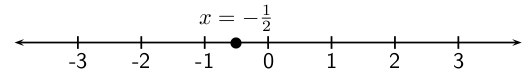
\includegraphics[width=.8\columnwidth]{col11306.imgs/m39254_MG10C10_001.png} % m39254;MG10C10\_001.png;;;6.0;8.5;
% \begin{center}
\begin{pspicture}(-4,0.75)(4,1.75)
%\psgrid
\psline[arrows=<->](-4,1)(4,1)
\psdot[dotsize=5pt](-0.5,1)
\multido{\n=-3+1}{7}
{\uput[d](\n,1){$\n$}
\psline(\n,1.1)(\n,0.9)}
\uput[u](-0.5,1){$x=-\frac{1}{2}$}
\end{pspicture}
% \end{center}
% \vspace{2pt}
% \vspace{.1in}
\end{center}
\end{figure}       
\par 
Kom ons los nou die ongelykheid $2x+2\leq1$ op:\par 


\begin{equation*}
\begin{array}{ccl}\hfill 2x+2& \leq& 1\hfill \\ \hfill 2x& \leq& 1-2\hfill \\ \hfill 2x& \leq& -1\hfill \\ \hfill x& \leq& -\frac{1}{2}\hfill \end{array}
\end{equation*}
As ons hierdie antwoord op ’n getallelyn voorstel, kry ons:\par 

\setcounter{subfigure}{0}
\begin{figure}[H] % horizontal\label{m39254*id157774}
\begin{center}
% \label{m39254*id157774!!!underscore!!!media}\label{m39254*id157774!!!underscore!!!printimage}
%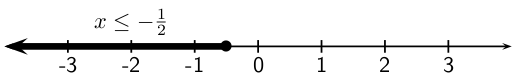
\includegraphics[width=.8\columnwidth]{col11306.imgs/m39254_MG10C10_002.png} % m39254;MG10C10\_002.png;;;6.0;8.5;
% \begin{center}
\begin{pspicture}(-4,0.75)(4,1.75)
%\psgrid
\psline[arrows=<->](-4,1)(4,1)
\psdot[dotsize=5pt](-0.5,1)
\multido{\n=-3+1}{7}
{\uput[d](\n,1){$\n$}
\psline(\n,1.1)(\n,0.9)}
\uput[u](-2,1){$x\leq-\frac{1}{2}$}
\psline[linewidth=3pt]{->}(-0.5,1)(-4,1)
\end{pspicture}
% \end{center}
% \vspace{2pt}
% \vspace{.1in}
\end{center}
\end{figure}       
\par 

% As ons hierdie oplossing in intervalnotasie uitdruk skryf ons $(-\infty ~;-\frac{1}{2}]$.\par
% \Note{Aanvaar $x \in \mathbb{R}$ as die versamelling getalle nie gespesifiseer word nie. }
Ons sien, vir die vergelyking is daar slegs ’n enkele waarde van  $x$ waarvoor die vergelyking waar is. Vir
die ongelykheid is daar egter ’n hele versameling waardes waarvoor die ongelykheid waar is. Dit is die groot
verskil tussen gewone vergelykings (gelykhede) en ongelykhede.\par 

\textbf{Onthou: } Wanneer beide kante van ’n ongelykheid met ’n negatiewe getal vermenigvuldig, of gedeel word, verander die rigting van
die ongelykheid. Om hierdie rede mag ons nie met ’n veranderlike vermenigvuldig as
ons nie weet nie wat die onbekende (veranderlike) se teken is nie.\par
\mindsetvid{Linear inequalities on a number line}{VMakv}

%english
\subsection*{Interval notation}
Examples:
\\
\begin{table}[H]
\begin{tabular}{|p{5cm}|p{8cm}|}
\hline
  $(4;12)$ &  Round brackets indicate that the number is not included. This interval includes all real numbers greater than but not equal to $4$ and less than but not equal to $12$.
\\ \hline
 $(- \infty; -1)$ & Round brackets are always used for positive and negative infinity. This interval includes all real numbers less than, but not equal to $-1$.
\\ \hline
 $[1; 13)$ & A square bracket indicates that the number is included. This interval includes all real numbers greater than or equal to $1$ and less than but not equal to $13$.
\\ \hline
\end{tabular}
\end{table}

It is important to note that this notation can only be used to represent an interval of real numbers. 

\par 
We represent the above answer in interval notation as $(-\infty;~-\frac{1}{2}]$.
\begin{wex}
{Los line\^ere ongelykhede op}
{
Los op vir $r$: $6-r>2$ \\
Stel jou antwoord voor op ’n getallelyn en in interval notasie.}
{ 
\westep{Herrangskik en los op vir $r$}  
\begin{equation*}
\begin{array}{ccl}\hfill -r&>&2-6\\ \hfill -r&>&-4\end{array}
\end{equation*}
%english
\westep{Multiply by $-1$ and reverse inequality sign}

\begin{equation*}
r<4
\end{equation*}

Onthou: wanneer ons met ’n negatiewe getal vermenigvuldig, draai die rigting
van die ongelykheid om.
\westep{Stel die oplossing voor op ’n getallelyn}

\setcounter{subfigure}{0}
\begin{figure}[H] % horizontal\label{m39254*id157937}
\begin{center}

%\includegraphics{col11306.imgs/m39254_MG10C10
% _003.png} % ;MG10C10\_003.png;;;6.0;8.5;
\begin{center}
\begin{pspicture}(-1,0.4)(6,1.6)
%\psgrid
\psline[arrows=<->](-1,1)(6,1)
\multido{\n=0+1}{6}
{\uput[d](\n,1){$\n$}
\psline(\n,1.1)(\n,0.9)}
\uput[u](2,1){$r<4$}
\psline[linewidth=3pt]{->}(4,1)(-1,1)
\psdot[dotsize=5pt,dotstyle=o](4,1)
\end{pspicture}
\end{center}

% \vspace{2pt}
% \vspace{.1in}
\end{center}
\end{figure}    

\westep{Druk die antwoord uit in intervalnotasie}
\begin{equation*}
(- \infty~;~4)   
\end{equation*}
}
\end{wex}

\begin{wex}{Los line\^ere ongelykhede op}
{
Los op vir $q$: $4q+3<2(q+3)$ \\
Stel die antwoord voor op 'n getallelyn en in intervalnotasie.
}
{
\westep{Brei die hakies uit}  
\begin{equation*}
\begin{array}{ccl}\hfill 4q+3& <& 2(q+3)\hfill \\ \hfill 4q+3& <& 2q+6\hfill \end{array}
\end{equation*}

\westep{Herrangskik en los op vir $q$}
\begin{equation*}
\begin{array}{ccl}\hfill 4q+3& <& 2q+6\hfill \\ \hfill 4q-2q& <& 6-3\hfill \\ \hfill 2q& <& 3\hfill \end{array}
\end{equation*}


\westep{Deel beide kante deur $2$}  
\begin{equation*}
\begin{array}{ccccc}\hfill 2q& <& 3\hfill &  \\ \hfill q& <& \frac{3}{2}\hfill & \end{array}
\end{equation*}

\westep{Stel die oplossing voor op ’n getallelyn} 

\setcounter{subfigure}{0}
\begin{figure}[H] 
\begin{center}
\begin{pspicture}(-1,0.4)(6,1.6)
%\psgrid
\psline[arrows=<->](-1,1)(6,1)
\multido{\n=0+1}{6}
{\uput[d](\n,1){$\n$}
\psline(\n,1.1)(\n,0.9)}
\uput[u](1,1){$q<\frac{3}{2}$}
\psline[linewidth=3pt]{->}(1.5,1)(-1,1)
\psdot[dotsize=5pt,dotstyle=o](1.5,1)
\end{pspicture}
\end{center}
\end{figure}   

\westep{Druk die antwoord uit in intervalnotasie}
\begin{equation*}
(- \infty~;~\frac{3}{2})
\end{equation*}
}
\end{wex}


\begin{wex}
{Los saamgestelde line\^ere ongelykhede op}
{Los op vir $x$: $5\leq x+3<8$ \\
Stel die oplossing voor op 'n getallelyn en in intervalnotasie.}  
{
\westep{Trek $3$ af van alle terme}
\begin{equation*}
\begin{array}{cccll}\hfill 5-3 &\leq& x+3-3 &<& 8-3\hfill \\
		  \hfill 2&\leq& x &<&5 \hfill
\end{array}
\end{equation*}

\westep{Stel die oplossing voor op ’n getallelyn.}

\setcounter{subfigure}{0}
\begin{figure}[H]
\begin{center}
\begin{pspicture}(-1,0.4)(6,1.6)
%\psgrid
\psline[arrows=<->](-1,1)(6,1)
\multido{\n=0+1}{6}
{\uput[d](\n,1){$\n$}
\psline(\n,1.1)(\n,0.9)}
\uput[u](3,1){$2\leq x < 5$}
\psline[linewidth=2.5pt](2,1)(5,1)
\psdot[dotsize=5pt,dotstyle=o](5,1)
\psdot[dotsize=5pt](2,1)
\end{pspicture}
\end{center}
\end{figure}       
}

\westep{Druk antwoord uit in intervalnotasie}
\begin{equation*}
[~2~;~5)
\end{equation*}
\end{wex}


\begin{exercises}{ }
{
Los op vir $x$ en stel die antwoord voor op 'n getallelyn en in intervalnotasie:
\begin{enumerate}[itemsep=6pt, label=\textbf{\arabic*}. ] 
    \item $3x+4>5x+8$
    \item $3(x-1)-2\leq 6x+4$ 
    \item $\dfrac{x-7}{3}>\dfrac{2x-3}{2}$
    \item $-4(x-1)<x+2$
    \item $\dfrac{1}{2}x+\dfrac{1}{3}(x-1)\geq \dfrac{5}{6}x-\dfrac{1}{3}$ 
    \item $-2\leq x-1<3$ 
    \item $-5<2x-3\leq7$ 
\item $7(3x+2)-5(2x-3)>7$
\item $\frac{5x - 1}{-6} \leq \frac{1-2x}{3}$
\item $3 \leq 4 - x \leq 16$
\item $\frac{-7y}{3} - 5 > -7$
\item $1 \leq 1 - 2y < 9$
\item $-2 < \frac{x-1}{-3}<7$
    \end{enumerate}

\practiceinfo

\par \begin{tabular}[h]{cccccc}
(1.) 00ea&  (2.) 00eb&  (3.) 00ec& (4.) 00ed& (5.) 00ee& (6.) 00ef& (7.) 00eg& (8.) 00eh & (9.) 022z & (10.) 0230 
& (11.) 0231 & (12.) 0232 & (13.) 0233 &\end{tabular}
}
\end{exercises}

\summary{M0001}


\begin{itemize}[noitemsep]
\item ’n Lineêre vergelyking is ’n vergelyking waar die hoogste mag van die veranderlike $1$. is. ’n Lineêre vergelyking het op die meeste een oplossing.
\item ’n Kwadratiese vergelyking is ’n vergelyking waar die hoogste mag van die veranderlike $2$ is. ’n Kwadratiese
vergelyking het op die meeste $2$ oplossings.
\item ’n Lineêre ongelykheid is soorgelyk aan ’n lineêre vergelyking en met die hoogste mag van die veranderlike
gelyk aan $1$.
\item Wanneer jy weerskante van ’n ongelykheid deel of vermenigvuldig met ’n negatiewe getal,
draai die rigting van die ongelykheid om. 
\item Wanneer twee onbekende veranderlikes opgelos moet word, moet jy twee vergelyking gebruik en hierdie vergelykings staan bekend as gelyktydige vergelykings. Daar is twee maniere waarop jy gelyktydige lineêre
vergelykings kan oplos: grafies en algebraïes om die vergelykings grafies op te los, trek jy ’n grafiek
van elke vergelyking en die oplossing sal die koördinate van die snypunt van die grafieke wees. Om die
oplossing algebraïes te vind, los jy een vergelyking op vir een veranderlike en stel dan daardie oplossing
in die ander vergelyking in om die tweede veranderlike se waarde te vind.
\item Lettervergelykings is vergelykings waar jy verskeie letters (veranderlikes) het en jy herrangskik die vergelyking om die oplossing te vind in terme van een van die letters (veranderlikes)
\item Wiskundige modellering (word probleme) is waar ons ’n vergelyking of ’n stel vergelykings opstel om ’n probleem wiskundig
voor te stel. Die oplossing van die vergelykings gee dan die oplossing van die probleem.
\end{itemize}

\begin{eocexercises}{}

 
\begin{enumerate}[itemsep=5pt, label=\textbf{\arabic*}. ] 
 \item 
Los op:
\begin{enumerate}[itemsep=6pt,label=\textbf{(\alph*)}]
\begin{multicols}{2} 
\item $2(p-1) = 3(p+2)$
\item $3-6k = 2k-1$
\item $m + 6(-m+1) + 5m = 0$
\item $2k + 3 = 2-3(k+3)$
\item $5t-1=t^{2}-(t+2)(t-2)$
\item $3+\dfrac{q}{5} = \dfrac{q}{2}$ 
\item $5-\dfrac{2(m+4)}{m} = \dfrac{7}{m}$
\item $\dfrac{2}{t} - 2 - \dfrac{1}{2} = \dfrac{1}{2}\left(1+\dfrac{2}{t}\right)$
\item $x^{2} - 3x + 2=0$
\item $y^{2} + y = 6$
\item $0=2x^{2} - 5x - 18$
\item $(d+4)(d-3)-d=(3d-2)^{2} - 8d(d-1)$
\item $5x+2\leq4(2x-1)$
\item $\dfrac{4x-2}{6} > 2x+1$
\item $\dfrac{x}{3} - 14 > 14 - \dfrac{x}{7}$
\item $\dfrac{1-a}{2} - \dfrac{2-a}{3} \geq 1$
\item $-5 \leq 2k + 1 < 5$
\item $x-1=\dfrac{42}{x}$  
\end{multicols}
\end{enumerate}

\item Beskou die volgende lettervergelykings:
\begin{enumerate}[itemsep=6pt,label=\textbf{(\alph*)}]
% \setcounter{enumi}{18}
\item Los op vir $I$: $P = VI$
\item Make $m$ the subject of the formula: $E=mc^{2}$
\item Los op vir $t$: $v = u + at$
\item Make $f$ the subject of the formula: $\dfrac{1}{u} + \dfrac{1}{v} = \dfrac{1}{f}$
\item Make $C$ the subject of the formula: $F=\frac{9}{5}C + 32$
\item Los op vir $y$: $m = \dfrac{y-c}{x}$
\end{enumerate}

\item Los die volgende stelsels gelyktydige vergelykings op:

\begin{enumerate}[itemsep=5pt,label=\textbf{(\alph*)}]
% \setcounter{enumi}{24}
\item $7x+3y=13$\\$2x-3y=-4$  
\item $10=2x+y$\\$y=x-2$
\item $7x-41=3y$\\$17=3x-y$
\item $2y=x+8$\\$4y=2x-44$
\end{enumerate}

\item Vind die oplossings van die volgende probleme:

\begin{enumerate}[itemsep=5pt,label=\textbf{(\alph*)}]
% \setcounter{enumi}{28}
\item $\frac{7}{8}$ van ’n getal is $5$ meer as $\frac{1}{3}$ van die getal. Vind die getal.

\item Drie liniale en twee penne kos saam R $21,00$. Een liniaal en een pen kos saam R
$8,00$. Hoeveel kos ’n pen op sy eie en hoeveel kos ’n liniaal op sy eie?

\item ’n Man hardloop na die busstop en terug in $15$ minutes. Sy spoed na die busstop is
$5$ km/h en sy spoed terug is $4$ km/h. Wat is die afstand na die busstop?
\item Zanele en Piet rolskaats na mekaar toe op ’n reguit pad. Hulle begin $20$ km van
mekaar af. Zanele skaars teen $15$ km/h en Piet teen $10$ km/h. Hoe ver sal Piet skaats
voor dat hulle by mekaar uitkom?

\item As die prys van sjokelade met R $10$ verhoog word, kan ons $5$ minder sjokelades
koop vir R $300$. Wat was die prys van elke sjokelade voor die prys verhoog het?

   

\end{enumerate}
\end{enumerate}
\practiceinfo
\par 
\par \begin{tabular}[h]{cccccc} 
(1a-f.) 00ei&  (1g-l.) 00ej& (1m-r.) 00ek&  (2a-f.) 00em&  (3a-d.) 00en&  (4a-e.) 00ep\end{tabular}

\end{eocexercises}